%!TEX root = ./HW2.tex

\section{25A Cities}
\subsection{Results}
For 25 cities in a ring, EA performs best.  All of the methods struggle with overcoming paths that go vertically across the circle.  Any single switch does not lead to a better solution.  Instead, multiple swaps are required to find a better solution.  Only MCTS might be able to overcome this; looking at the solution, it seems that it is approaching a better solution, but did not have enough iterations.

The distribution of the cities affects the solution quality.  For the ring, switching two consecutive cities is all that is needed for a better solution.  This does not apply when two consecutive cities are directly across the the Y direction of the circle.  The ovalness of the distrution means directly adjacent cities are not closer.  This is a local minimum which is hard to escape.  A similar problem can be observed in the other 25 city distribution.  However, here the lack of structure in the solution makes many of the switches not as productive.  Instead, multiple consecutive city switches are required to find a better solution.  This makes the problem more challenging.  
\begin{table}[H]
\centering
\begin{tabular}{|c|c|c|c|c|c|}
\hline
Algorithm               & \begin{tabular}[c]{@{}c@{}}Total Solutions\\ Generated\end{tabular} & \begin{tabular}[c]{@{}c@{}}Average Min\\ Distance\end{tabular} & St Dev & \begin{tabular}[c]{@{}c@{}}Average\\ Run Time (s)\end{tabular} & St Dev  \\ \hline
Simulated Annealing     & 10,000                                                              & 13,796                                                         & 1,742  & 3.70e-6                                                        & 8.94e-7 \\ \hline
Evolutionary Algorithm  & 10,000                                                              & 12,222                                                         & 1,337  & 9.89                                                           & 0.03    \\ \hline
Monte Carlo Tree Search & 10,000                                                              & 12,047                                                         & 937    & 3.70                                                           & 0.15    \\ \hline
\end{tabular}
\caption{Comparison of Solution Quality and Run Time for Each Method with 25 Cities}
\label{tab:25Comparison}
\end{table}

% insert image of example solutions found by search

\begin{figure}[H]
	\centering
    \begin{minipage}{0.45\textwidth}
        \centering
        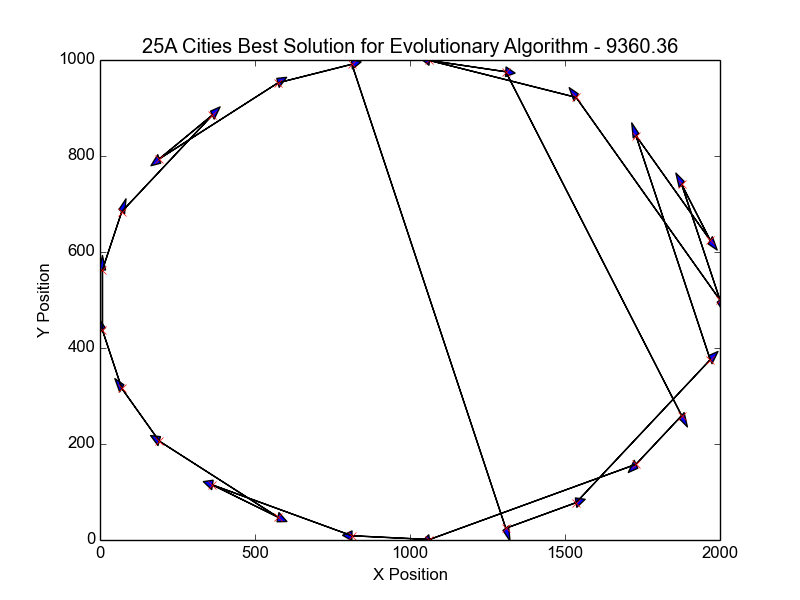
\includegraphics[width=0.9\textwidth]{25ACity_EA.png} % first figure itself
        \caption{Best Solution for 25A Cities with Evolutionary Algorithm}
        \label{fig:25Acity_EA}
    \end{minipage}\hfill
    \begin{minipage}{0.45\textwidth}
        \centering
        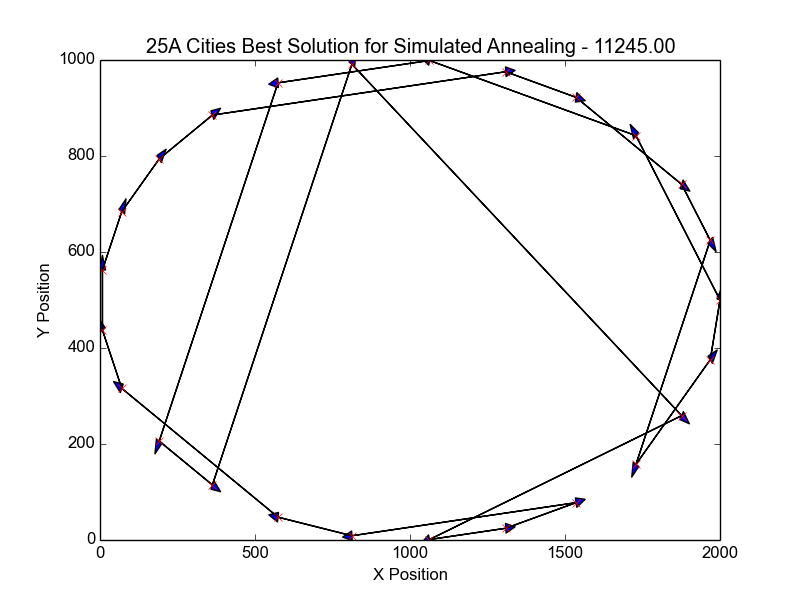
\includegraphics[width=0.9\textwidth]{25ACity_SA.png} % second figure itself
        \caption{Best Solution for 25A Cities with Simulated Annealing}
        \label{fig:25Acity_SA}
    \end{minipage}\hfill
    \begin{minipage}{0.45\textwidth}
        \centering
        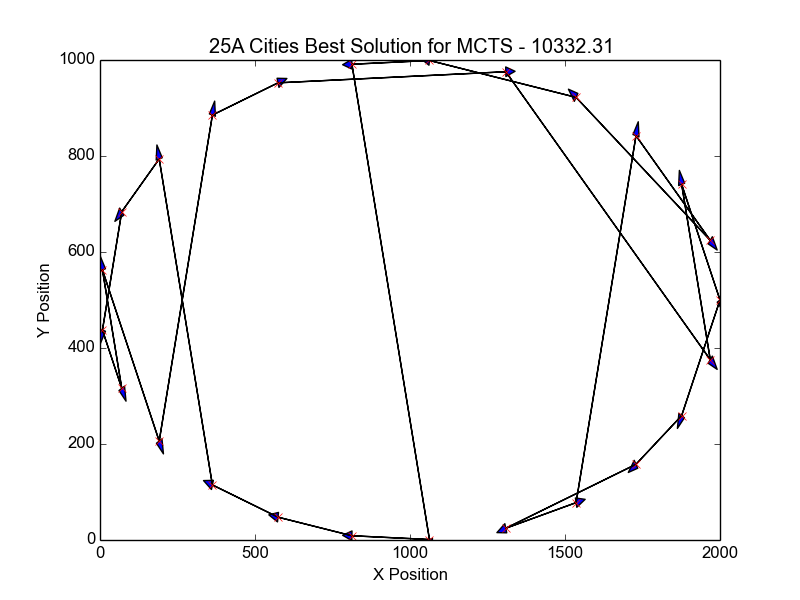
\includegraphics[width=0.9\textwidth]{25ACity_MCTS.png} % third figure itself
        \caption{Best Solution for 25A Cities with MCTS}
        \label{fig:25Acity_MCTS}
    \end{minipage}\hfill
    \begin{minipage}{0.45\textwidth}
		\centering
		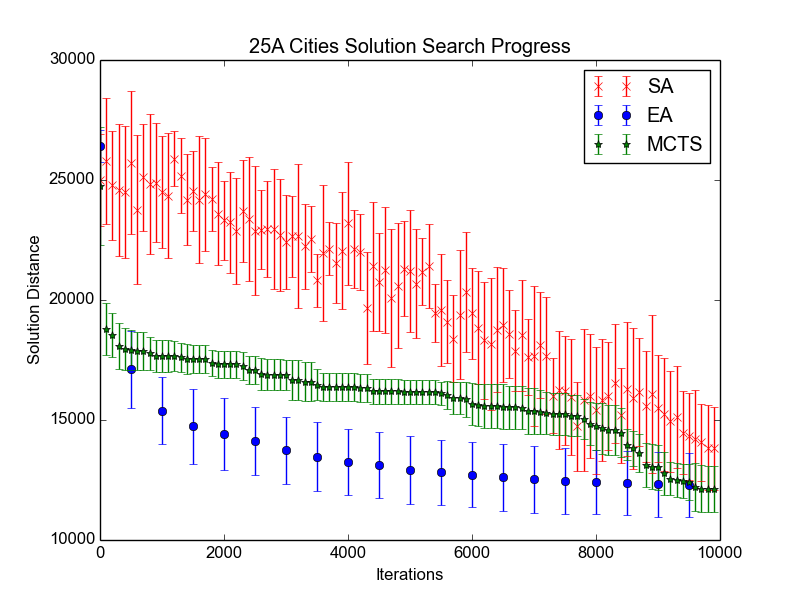
\includegraphics[width=0.9\textwidth]{25ACity_Solutions.png}
		\caption{Solution Progression for 25A Cities}
		\label{fig:25Acity_Solution}
    \end{minipage}\hfill
\end{figure}